\documentclass[paper=a4, fontsize=11pt]{article} % A4 paper and 11pt font size
\usepackage[utf8]{inputenc}
\usepackage[T1]{fontenc} % Use 8-bit encoding that has 256 glyphs
\usepackage{fourier} % Use the Adobe Utopia font for the document - comment this line to return to the LaTeX default
\usepackage[ngerman,british,UKenglish,USenglish,american]{babel}
\usepackage[utf8]{inputenc}
\usepackage{amsmath,amsfonts,amsthm} % Math packages
\usepackage{hyperref}
\usepackage{fancyhdr}
\usepackage{graphicx}
\usepackage{listings}
\usepackage{todonotes}
\usepackage{titlesec}
\usepackage{xcolor}
\usepackage{ulem}
\definecolor{grey}{rgb}{0.4, 0.4, 0.4}

%\usepackage{sectsty} % Allows customizing section commands
%\allsectionsfont{\centering \normalfont\scshape} % Make all sections centered, the default font and small caps

\usepackage{fancyhdr} % Custom headers and footers
\pagestyle{fancyplain} % Makes all pages in the document conform to the custom headers and footers
\fancyhead[R]{} % No page header - if you want one, create it in the same way as the footers below
\fancyfoot[L]{} % Empty left footer
\fancyfoot[C]{\thepage} % Page numbering for center footer
\fancyfoot[R]{} % Empty right footer
\renewcommand{\headrulewidth}{0pt} % Remove header underlines
\renewcommand{\footrulewidth}{0pt} % Remove footer underlines
\setlength{\headheight}{13.6pt} % Customize the height of the header

%farbige Hyperlinks
%\definecolor{refcolor}{rgb}{0,.2,.4}
%schwarze Hyperlinks
\definecolor{refcolor}{rgb}{0,0,0}
%Hyperref Color
\hypersetup{pdftex=true, colorlinks=true, breaklinks=true, linkcolor=refcolor, menucolor=refcolor, pagecolor=refcolor, citecolor=refcolor, urlcolor=blue}

\numberwithin{equation}{section} % Number equations within sections (i.e. 1.1, 1.2, 2.1, 2.2 instead of 1, 2, 3, 4)
\numberwithin{figure}{section} % Number figures within sections (i.e. 1.1, 1.2, 2.1, 2.2 instead of 1, 2, 3, 4)
\numberwithin{table}{section} % Number tables within sections (i.e. 1.1, 1.2, 2.1, 2.2 instead of 1, 2, 3, 4)

\setlength\parindent{0pt} % Removes all indentation from paragraphs - comment this line for an assignment with lots of text
% Code Listing Style
\definecolor{darkblue}{rgb}{0,0,.6}
\definecolor{darkgreen}{rgb}{0,0.5,0}
\definecolor{darkred}{rgb}{0.5,0,0}
\lstset{
	basicstyle=\ttfamily,
	commentstyle=\color{darkgreen},
	keywordstyle=\color{darkblue}\fontseries{sb}\fontshape{n}\selectfont,
	stringstyle=\color{darkred},
%	identifierstyle=\color{darkgreen},
%    moredelim=[is][\underbar]{_}{_},
	breaklines=true,
	tabsize=2,
%	xleftmargin=-1mm,
%	xrightmargin=3mm,
%	aboveskip=\smallskipamount,
%	belowskip=\smallskipamount,
	numbers=none,
	frame=none,
	showstringspaces=false,
	captionpos=t,
%	framexbottommargin=3pt,
%	framextopmargin=3pt,
	% Umlaute
	literate=%
		{Ö}{{\"O}}1
		{Ä}{{\"A}}1
		{Ü}{{\"U}}1
		{ß}{{\ss}}2
		{ü}{{\"u}}1
		{ä}{{\"a}}1
		{ö}{{\"o}}1
}

% BibLaTeX
%\usepackage[style=authoryear]{biblatex}
%\usepackage[style=numeric]{biblatex}
\usepackage[style=alphabetic]{biblatex}

\AtEveryBibitem{\clearlist{language}} % clears language
\AtEveryBibitem{\clearfield{note}}    % clears notes
\AtEveryBibitem{\clearfield{doi}} % clears doi
\AtEveryBibitem{\clearfield{isbn}} % clears doi
\AtEveryBibitem{\clearfield{issn}} % clears doi
\addbibresource{bibliography.bib} % Syntax for version >= 1.2

%----------------------------------------------------------------------------------------
%	TITLE SECTION
%----------------------------------------------------------------------------------------

\newcommand{\horrule}[1]{\rule{\linewidth}{#1}} % Create horizontal rule command with 1 argument of height

\title{	
\normalfont \normalsize 
\textsc{\includegraphics[width=0.6\textwidth]{pictures/logo} \\ [5pt] Arbeitsgruppe Datenbanken und Informationssysteme \\ [20pt] \includegraphics[width=0.15\textwidth]{pictures/DBIS_Logo_rgb_web.png}} \\ [10pt] % Your university, school and/or department name(s)
\horrule{0.5pt} \\[0.4cm] % Thin top horizontal rule
\huge Spatial Databases: Project Documentation \\ % The assignment title
\normalsize \textsc{Setup-Guide and Documentation for Spatial-Weather-Project} \\ [0.4cm]
\horrule{2pt} \\[0.5cm] % Thick bottom horizontal rule
}
\newcommand*{\justifyheading}{\raggedright}
\titleformat{\subsection}{\large\justifyheading}{\thesubsection}{1em}{}

\author{Johannes Dillmann (4476004) \\ Christian Wirth (4498611) \\ Jens Fischer (3923671)}

\date{\normalsize\today} % Today's date or a custom date
\begin{document}

\begin{titlepage}
\pagenumbering{Roman}
\maketitle
\thispagestyle{empty}
\end{titlepage}

\newpage
\setcounter{page}{1}
\addcontentsline{toc}{section}{\protect\numberline{}{Table of Contents}}
\tableofcontents
%\thispagestyle{empty}

\newpage
\listoffigures
\addcontentsline{toc}{section}{\protect\numberline{}{Table of Figures}}

\newpage
\pagenumbering{arabic}
\pagestyle{fancy}
\setcounter{page}{1}

\section{Introduction}
	\subsection{Topic}
	The topic of this project is to combine OSM-data provided by Open Street Maps and weather-Data on a spatial database server running PostGIS.
	\subsection{Motivation}
	The motivation of this project can be seen from a educational as well as from a technical point of view.\\
	The educational purpose of this project is to encourage the students to acquire domain-knowledge concerning the problem that needs to solved with a system that is requested to be set up. In this particular case the domain is weather-data. By working hands-on with real data the students expand their range of skills in order to be able to work with problems that exceed the boundary of purely computational and mathematical problems. This focuses on an important trade every programmer will need once he leaves university and has to deal with real world problems.\\
%	Once these domain-related problems are understood the students face the technological challenges in order to find a solution to the given problem which will be explained in the following subsection.
% zu Anti-Uni, das findet Voisard nicht gut
	\subsection{Goal}
	The Goal is to find suitable sources for weather-forecast and historical weather-data as well as storing it on a PostGIS-server. In the end the system shall be able to overlay the OSM- and the collected weather data. In order to achieve this goal several technical problems have to be solved, like designing a data model, a suitable system architecture as well as setting up and configuring the whole system.
	
\newpage
\section{Data Sources}\label{sec:datasources}

We are using three differente data sources for administrative borders, historical
and forecast weather data. Since the historical data is feature based but the
forecasts are provided as regular grid, we decided to use irregular tesselation to display
weather information for german states and districts and a voronoi diagram based
on official german weather stations. 

\subsection{Deutscher Wetterdienst (DWD)}
The DWD provides historical meassurement data from 509 weather stations all over 
germany. The data is freely available as comma-separated values (CSV) from a FTP
server. Every station is identified by a unique id, has a name, a spatial location
and an altitude and provides multiple daily meassurements.

As mentioned above we use the stations locations to generate a voronoi tesselation
covering germany and assign each resulting cell the meassurement from the associated 
station. To get values for districts or states, we are calculating a weighted mean
based on the area a voronoi cell is contributing. Since this operation is costly
we did apply some optimisations as described in section \ref{subsec:opticontrib}.

The tool used to download and import DWD data is based on work of a fellow student
working on the same topic \todo{quelle stat link} \url{https://github.com/cholin/fuberlin_spatial_db_project}.
Its usage is described in section \ref{import-dwd-data}.


\subsection{Global Forecast System (GFS)}
We use data from the Global Forecast System (GFS) in our application for weather 
forecasts. The GFS is a weather forecast model computed and freely distributed
by the National Oceanic and Atmospheric Administration (NOAA) of the United States.


The GFS model is calculated every 6h hours and covers the entire globe at a resolution 
of 28 kilometers for weather predictions within 16 days. Furthermore it provides
forecast up to two weeks with a lower resolution of 70 kilometers. 


The data is free is free of charge an can be downloaded as Gridded Binaries (GRIB) 
from the NOAA servers. They provide among other access methods like FTP services, 
a simple \href{http://nomads.ncep.noaa.gov/txt_descriptions/grib_filter_doc.shtml}{webinterface}
to extract certain levels and variables for a subregion.


Because we are only interested in the temperature and rainfall forecasts for 
Germany, we are using that interface to download the GRIB data. Because the 
webinterface does not allow to download data older than one month, we provide 
separate download and import scripts as described in section \ref{download-and-import-noaa-gfs-data-forecasts} 
that can be run periodically. 

\subsection{OpenStreetMap (OSM)}
OSM is used to get the administrative borders of Germany, german states and districts.
Since we are using tiles from external providers, we didn't have to render them 
ourselves from the OSM data. We recommend to download compressed PBF files 
for Germany from Geofabrik and import them with imposm as described in section \ref{import-osm-data}.


\section{Data Model}

\subsection{Entity Relationship Diagram (ERD) }
  \begin{figure}[htbp]
  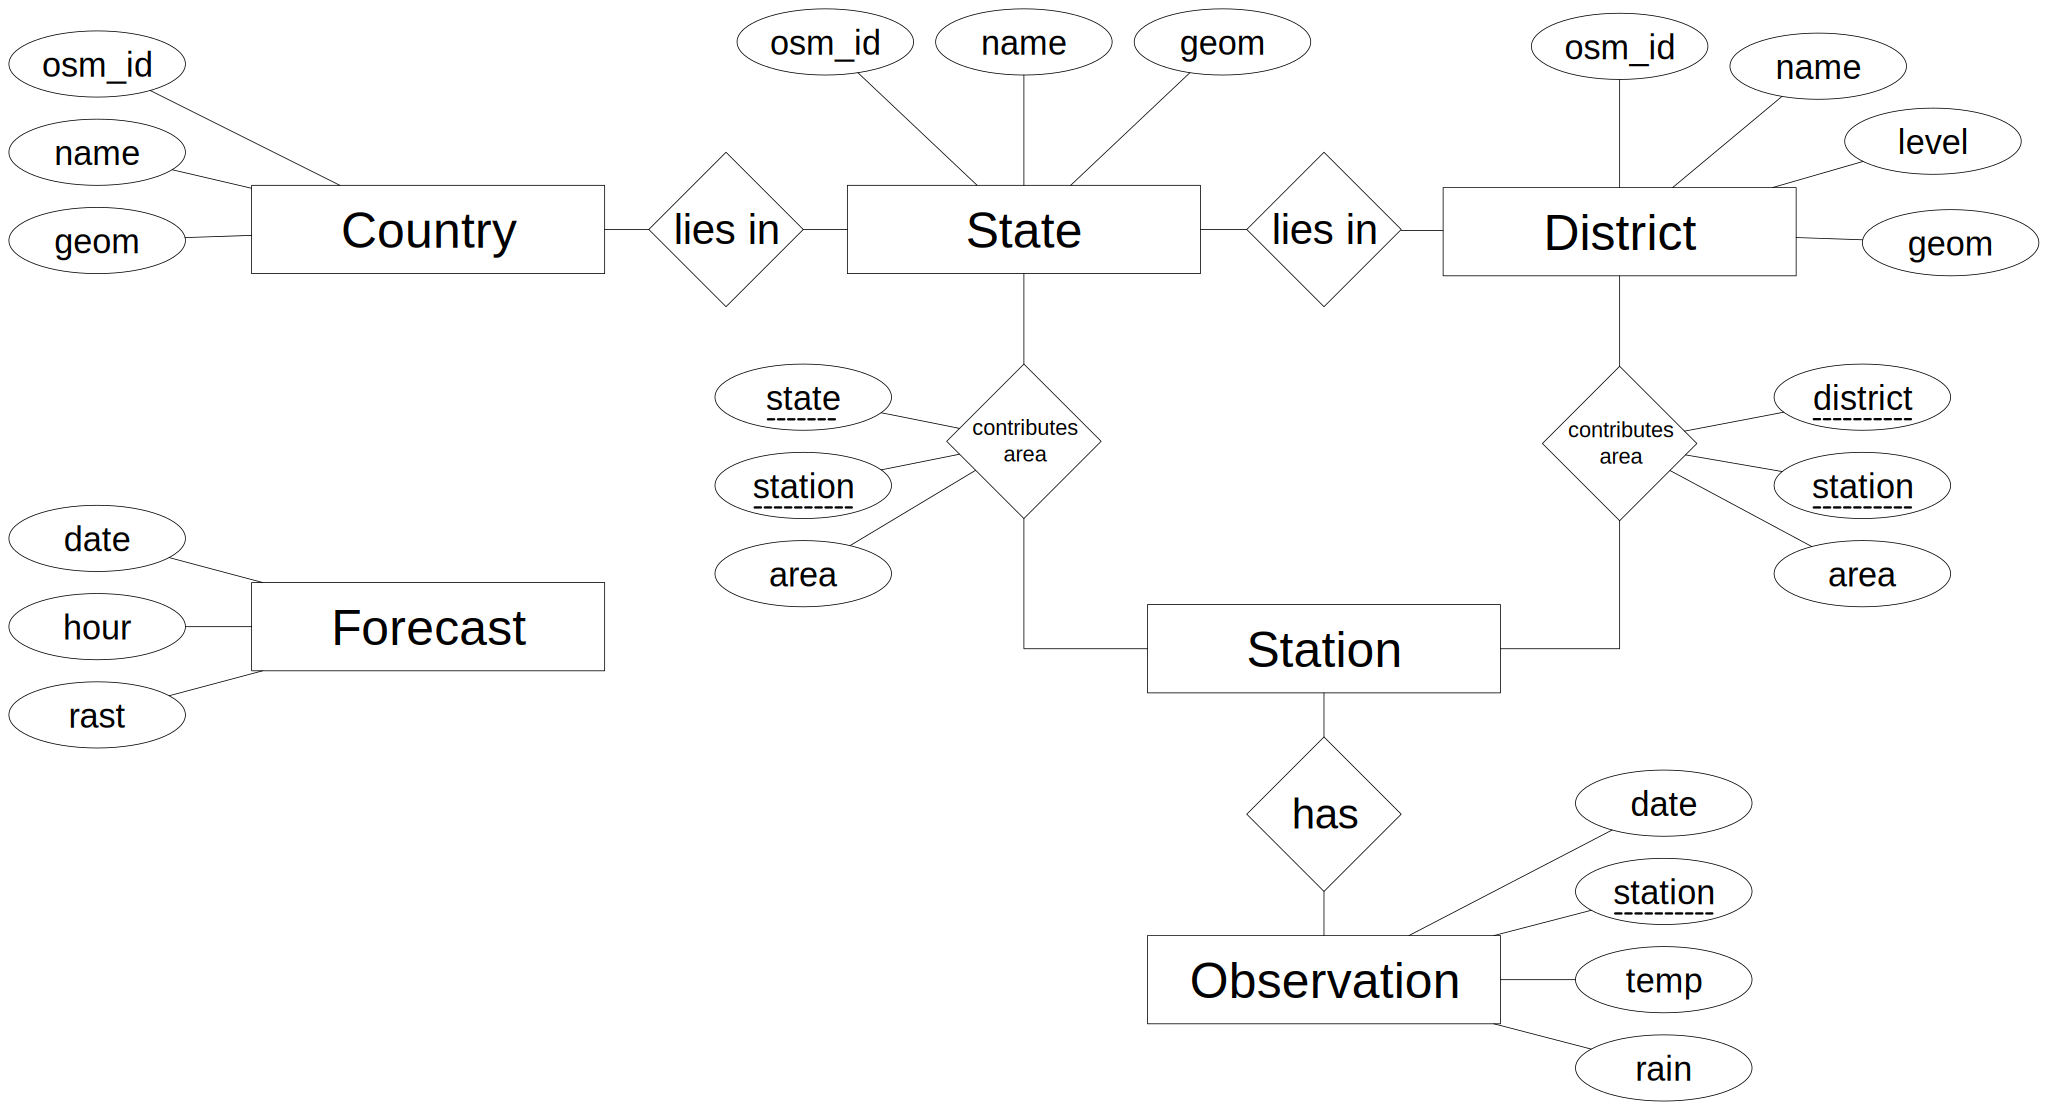
\includegraphics[width=1\textwidth]{pictures/er-model}
  \caption{ER-Diagram}
  \end{figure}

\subsection{Relational Schema}
  
  Country : \{{[}\uline{osm\_id: biginteger}, name: string, geom:  geometry{]}\}

  State : \{{[}\uline{osm\_id: biginteger}, name: string, geom: geometry{]}\}

  District : \{{[}\uline{osm\_id: biginteger}, name: string, geom: geometry{]}\}

  Station : \{{[}\uline{dwd\_id: integer}, name: string, altitude: integer, geometry: point, region: geometry{]}\}

  Observation : \{{[}\uline{\dashuline{station\_id: integer}, date: timestamp}, temperature: double, rainfall: double{]}\}

  Forecast : \{{[}\uline{date: timestamp, hour: integer}, rast: raster{]}\}

  ContribState : \{{[}\uline{\dashuline{state\_id: biginteger}, \dashuline{station\_id: integer}}, area: double{]}\}

  ContribDistrict : \{{[}\uline{\dashuline{district\_id: biginteger}, \dashuline{station\_id: integer}}, area: double{]}\}

  ~\\
  The relational schema is following \textcite{Kemper2011}. The schema is not identical to the schema used in the actual PostgreSQL DB where for example additional fields used solely for the import are still remaining. The presented schema is given for illustrating conceptual ideas. 
  
  ~\\
  As can be seen in the relational schema there are no foreign keys or junction tables
  used to reference the relation between countries, states, districts and stations. 
  Those entities are related by their spatial component and will be joined by using
  spatial joins provided by the PostGIS extension. 





\newpage
\section{Architecture}
The architecture as shown in fig. \ref{fig:architecture} consist of 4 major parts:\\
The data sources and their corresponding downloaders and importers, the PostGIS-Server, running in a virtual machine, the backend and a webapp. In the following four subsections \ref{subsec:dsai} to \ref{subsec:webapp} it will be  explained how those components work together and what parts they are made of as well as which technologies have been used to implement them.
\begin{figure}[htbp]
\includegraphics[width=1\textwidth]{pictures/Architektur.png}
\caption{Architecture}
\label{fig:architecture}
\end{figure}
\todo[inline]{Schreibfehler korrigieren}

\subsection{Data Sources and Importer}\label{subsec:dsai}
The three data-sources used in this project are \todo[inline]{add 3 sources} and have been discussed in section \ref{sec:datasources} very detailed. The importers write the collected data directly to the spatial database server so they can be used to answer the queries by the backend. For further information on this part please refer to section \ref{sec:datasources} and the setup-guide at subsections \ref{import-osm-data} to \ref{download-and-import-noaa-gfs-data-forecasts}
\subsection{Database Server}
The database server is provided as Vagrant virtual machine. Vagrant is a tool to automate the setup of virtual machines. In this case vagrant initializes a Ubuntu x64 instance and installs postgres and PostGis along with other required packages and configures most of the things needed for the server to be used.
\subsection{Backend}
The backend runs Flask, a model-view-controller-based web framework. This framework contains methods to invoke data collection and data import as well as an ORM based on SQLAlchemy and GEOAlchemy to send queries to the database to retrieve data requested by the user via the frontend. The queries are written in python, the ORM translates those queries to SQL and the the response from the database is converted to GeoJSON, which is then forwarded to the frontend.
\subsection{Webapp (Frontend)}\label{subsec:webapp}
The frontend in implemented as a webapp written in HTML5, CSS3 and Javascript and provides a user interface which is described in detail in section \ref{usage}. To display the weather and OSM data the library Leaflet is used. The frontend receives the requested data from the backend in (Geo)JSON.

\section{Optimisations}

\subsection{Indices}

Indices were used on all primary keys, all geometry columns and some frequently queried attributes, like dates. All indices were used from the beginning, so no information on the performance gains is available.

\subsection{Materialised Computations}\label{subsec:opticontrib}

When querying the forecast information for all the states, districts or stations our first implementation used nested queries within the ORM (i.e. multiple queries where send to the database). This queries took extremely long, several minutes in the case of districts. To improve performance, we reimplemented this query as one nested query (i.e. the nesting was done \emph{within} one query). This already improved performance significantly. But we also noted that one of the nested subqueries was basically a static computation, namely the computation of the area contribution of the region of a weather station (i.e. the Voronoi cell of a weather station) to the area of a state or district. Therefore we decided to materialise this computation into two tables (\lstinline{Contrib_State}, \lstinline{Contrib_District}), which brought down the query time significantly. 

\subsection{Border Simplifications}	

When profiling the application further, we noticed that the huge amount of detail of the country, state and district borders seriously affected the performance, not only in terms of querying but also the sheer amount of data transmitted from the server to the client. 

Initially, after the import from Open Street Maps, all the country, state and district geometry columns had a combined size of 38 MiB. In an attempt to further improve performance we wanted to simplify the geometries, especially as they were only used for querying and overlaying the respective regions, not for the rendering of the map itself.

The main problem here is that the simplification needs to preserve the topological relationships between the different polygons. Postgis provides the function \lstinline{ST_Simplify}, but this function works on an object-by-object basis. Using this to simplify the borders produces holes and overlaps between the borders. Although the name seems to indicate otherwise, \lstinline{ST_SimplifyPreserveTopology} doesn't solve the problem (it only tries to preserve topologic relationships of multilines and multipolygons).

The way to achieve simplification and preserve topological relationships is to use the topology feature of Postgis. This means to create a topology, add a layer for the borders, populate the topology from the polygons, simplify the borders within the topology and convert the borders back to polygons. This method was adapted from \textcite{website:strks-blog}. The complete Script can be found in the Apendix. Figure \ref{borders_full}, \ref{borders_simple}, \ref{germany_full} and \ref{germany_simple} compare the effects of the simplification. We aimed at achieving meaningful reduction in size but still maintain the basic characteristics of the borders. As one can see at fig. \ref{borders_full} and \ref{borders_simple}, on the smallest level the differences in detail are clearly notable. When looking at a larger zoom level, as in fig. \ref{germany_full} and \ref{germany_simple}, one can hardly spot the difference. To total combined size of the geometry columns after the simplification was 895 KiB! A further optimisation could be to provide different levels of detail for different zoom levels.

\begin{figure}[htbp]
	\centering
	\includegraphics[trim = 0mm 0mm 0mm 0mm, clip, width=0.95\textwidth]{pictures/berlin_full}
	\caption{Berlin Full Detail}
	\label{borders_full}
\end{figure}

\begin{figure}[htbp]
	\centering
	\includegraphics[trim = 0mm 0mm 0mm 0mm, clip, width=0.95\textwidth]{pictures/berlin_simplified}
	\caption{Berlin Simplified}
	\label{borders_simple}
\end{figure}

\begin{figure}[htbp]
	\centering
	\includegraphics[trim = 160mm 0mm 160mm 0mm, clip, width=1\textwidth]{pictures/germany_full}
	\caption{Germany Full Detail}
	\label{germany_full}
\end{figure}

\begin{figure}[htbp]
	\centering
	\includegraphics[trim = 160mm 0mm 160mm 0mm, clip, width=1\textwidth]{pictures/germany_simplified}
	\caption{Germany Simplified}
	\label{germany_simple}
\end{figure}



Figure \ref{simplification_table} summarises the performance gains for the most intensive query we perform. As you can see, the simplification achieved significant performance improvements.

\begin{figure}[htbp]
	\centering
	\includegraphics[trim = 0mm 0mm 0mm 0mm, clip, width=1.1\textwidth]{pictures/simplification_table}
	\caption{Performance Gains From the Simplification}
	\label{simplification_table}
\end{figure}


\section{Usage}\label{usage}

As mentioned in the architecture section, the weather map is displayed
with HTML5 and controlled with JavaScript. It has been developed as a
control for the Leaflet library and tested on Google Chrome and
Chromium. Other browsers are not officially supported.

By default Leaflet is using a zoom and a layer selection control.
Instead of rendering the base tiles ourselves, we are using the freely
available
\todo[inline]{Sources}
\href{http://wiki.openstreetmap.org/wiki/Tile_usage_policy}{OSM Tile
Server} and tiles generated for free by
\href{https://www.mapbox.com/}{Mapbox}. The desired basetile layer can
be selected as seen in fig. \ref{fig:layer-selection}.
The map can also be panned and zoomed by using a pointing device
(e.g. mouse).

\begin{figure}[htbp]
\includegraphics[width=1\textwidth]{pictures/screenshot-baselayer.png}
\caption{Layer selection}
\label{fig:layer-selection}
\end{figure}

The displayed weather data can be set by an additional control as seen
in fig. \ref{fig:weather-control}.
It allows to choose either temperatures or reciprocal rainfall for a
certain day. The day can be selected with an interactive date-time picker
as seen in fig. \ref{fig:date-time-picker}.

\begin{figure}[htbp]
\includegraphics[width=1\textwidth]{pictures/screenshot-control.png}
\caption{Weather control}
\label{fig:weather-control}
\end{figure}

\begin{figure}[htbp]
\centering
\includegraphics[width=1\textwidth]{pictures/screenshot-control-datetime.png}
\caption{Date-time picker}
\label{fig:date-time-picker}
\end{figure}

The selected date and time is also used to pick the computed GFS used to
display forecasts. If the forecast box is checked, the forecasts slider
is activated and allows to select point of forecast in hours, starting
from the chosen date and time.

As mentioned before, the data can be displayed for different rasters: a
voronoi tessellation based on official weather stations, german states or
districts as shown in fig. \ref{fig:raster-comparison}. The desired raster can be selected with the control. Once the
selection did change, the weather control is loading the matching data
from the backend via a JSON interface and displays the raster on the
map.

The cells are colored according to selected data and a legend is shown
on the lower right for reference (see fig. \ref{fig:temperature-legend} and \ref{fig:rainfall-legend})

\begin{figure}[htbp]
\centering
\includegraphics[width=1\textwidth]{pictures/screenshot-raster.png}
\caption{Raster comparison}
\label{fig:raster-comparison}
\end{figure}

\begin{figure}[htbp]
\centering
\includegraphics[width=0.5\textwidth]{pictures/screenshot-legend-temp.png}
\caption{Temperature legend}
\label{fig:temperature-legend}
\end{figure}

\begin{figure}[htbp]
\centering
\includegraphics[width=0.5\textwidth]{pictures/screenshot-legend-rain.png}
\caption{Rainfall legend}
\label{fig:rainfall-legend}
\end{figure}

\newpage
Each cell is clickable and highlights it's border or, in case of the
voronoi tessellation, the position of the weather station. Furthermore a
pop-up as in fig. \ref{fig:popup} is shown, which provides additional data associated to the
selected cell by calling the backends JSON interface.

Currently this is just the alphanumerical attributes, but could be used
to show automatically generated temperature timelines or recent webcam
photos. \todo[inline]{noch mehr ausblick kram\ldots}

\begin{figure}[htbp]
\centering
\includegraphics[width=1\textwidth]{pictures/screenshot-popup.png}
\caption{Pop-up}
\label{fig:popup}
\end{figure}

\section{Conclusion}
	- lessons learned










\section{Setup Guide}
\subsection{Prerequisites}

This Setup-Guide has been writen for and tested with Ubuntu 14.10 'Utopic Unicorn'.\\
The Following Packages or Programs need to be installed before you proceed with this set-up-guide: Git, Vagrant, Python 3, PostGIS and the postgres database drive for Python.

\begin{lstlisting}
sudo apt-get install gdal-bin postgis git vagrant python3 python3-dev python3-psycopg2 libpq-dev 
\end{lstlisting}

It is strongly advised to install scipy, numpy and shapely (globaly) as
binary packages and not through virtualenv, because of their large
number of non-python dependencies. E.g. on Debian/Ubuntu systems use
\begin{lstlisting}
sudo apt-get install python3-numpy python3-scipy python3-shapely 
\end{lstlisting}
to install. Make sure access to the global packages is activated in the
virtual environment.

When compiling entirely from source, You also might need to install the
following libraries: (for shapely): libgeos-dev; (for scipy):
libblas-dev, liblapack-dev, gfortran.

\subsection{Step-by-step Setup}
Now switch to directory that should later contain your project-source-code

\todo[inline]{Auf Github verweisen}
Clone Repository by typing into console:
\begin{lstlisting}
git clone https://github.com/jvf/spatial-weather.git
\end{lstlisting}

Change directory to spatial-weather
\begin{lstlisting}
cd spatial-weather
\end{lstlisting}

Install and configure the virtual machine by entering in console:
\begin{lstlisting}
vagrant up
\end{lstlisting}

You can open a new console and proceed with the following steps on your local machine:\\
Install miniconda from the website: 
\url{http://conda.pydata.org/miniconda.html} and create a virtual environment with the following command:

\begin{lstlisting}
conda create -n spatial-weather --file requirements.conda
\end{lstlisting}

The virtual environment can be activated by executing the following command.
Remember that the environment has to be active to start the server succesfully.
\begin{lstlisting}
source activate spatial-weather
\end{lstlisting}

The first time the environment is activated it is required to install additional 
requirements that are not available within the conda distribution. The installation
is handled by pip and can be called with the following command. 
\begin{lstlisting}
pip install -r requirements.txt
\end{lstlisting}

The weather app requires a databse with the postgis and postgis\_topology extensions enabled.
The following command can be used to create the default database with the required
access levels within the previously provisioned virtual machine.
\begin{lstlisting}[breaklines=true]
vagrant ssh -c "sudo -u postgres psql -c \"CREATE DATABASE spatial OWNER myapp LC_COLLATE 'en_US.UTF-8' LC_CTYPE 'en_US.UTF-8';\"" 
vagrant ssh -c "sudo -u postgres psql -d spatial -c \"CREATE EXTENSION postgis; CREATE EXTENSION postgis_topology;\"" 
vagrant ssh -c "sudo -u postgres psql -d spatial -c \"GRANT ALL ON DATABASE spatial TO myapp; ALTER DATABASE spatial OWNER TO myapp; ALTER TABLE topology OWNER to myapp; ALTER TABLE layer OWNER to myapp; ALTER SCHEMA topology OWNER TO myapp;\""
\end{lstlisting}

\subsection{Import OSM Data}\label{import-osm-data}

Imports the OSM data for Germany. The following tables are created: Country, State, District and Cities. The data is imported from \texttt{germany-latest.osm.pbf}, which can be obtained from \href{http://download.geofabrik.de/europe/germany-latest.osm.pbf}{Geofabrik}. The pbf file needs to be placed in \texttt{data/} located in your Project-Folder.

The importer used is \texttt{imposm3}, which is included in the vagrant setup (and will be executed within the VM). The import uses a custom mapping, which is provided in \texttt{importer/mapping.json}. The import is conducted in two steps: First, the data is imported to the tables Osm\_Admin and Osm\_Places. Second the Country, State, District and Cities tables are created from these tables.

\subsubsection*{Usage}\label{usage}

Prerequisite: No contrib tables, delete if existing:
\begin{lstlisting}
	python manage.py drop_tables -t contrib
\end{lstlisting}

To import all the OSM data use the manage script. To invoke the whole pipeline use the following command (will take several hours):

\begin{lstlisting}
	python manage.py import_osm --imposm --simplify --load --drop_tables	
\end{lstlisting}


\begin{itemize}
\itemsep1pt\parskip0pt\parsep0pt
\item
  \texttt{-\/-imposm} the first import step (see above)
\item
  \texttt{-\/-simplify} simplify all map data (borders)
\item
  \texttt{-\/-load} the second import step (see above)
\item
  \texttt{-\/-drop-tables} deletes the Osm\_Admin and Osm\_Places tables
  after a successful import
\end{itemize}

All the above steps can be invoked separately.

\subsection{Import DWD Data (Historical Weather Data)}\label{import-dwd-data}

Imports weather observation data from the DWD (Deutscher Wetterdienst).
The importer is a adopted version from \textcite{website:cholin} . Per default, it downloads all the \href{ftp://ftp.dwd.de/pub/CDC/observations_germany/climate/daily/kl}{recent daily
observations}. Details on the importer from \textcite{website:cholin}:

\begin{quote}
The importer downloads the station summary file to get a list of all weather stations. After that it downloads for each station the corresponding zip file (with measurement data), extracts it in-memory and parses it. To get information about which weather station is the nearest for a given point, it also calculates a region polygon for each station. This is done by computing the voronoi diagram for all stations. The resulting regions may be outside of the country germany. To avoid this there is a polygon of the border of germany (data is from naturalearthdata.com - country extraction and exportation as geojson with qgis). For each region we calculate the intersection with this polygon and use the result as final region (Multi)Polygon.
\end{quote}

\subsubsection*{Usage}\label{usage-1}

Use the importer with the \texttt{manage.py} script:

To download all data and import all observation data:

\begin{lstlisting}
	python manage.py import_dwd
\end{lstlisting}


Create an intermediate result in \texttt{data/weather.json}:

\begin{lstlisting}
	python manage.py import_dwd --to_json
\end{lstlisting}


Import the intermediate result from \texttt{data/weather.json}:

\begin{lstlisting}
	python manage.py import_dwd --from_json
\end{lstlisting}


\subsection{Download and Import NOAA GFS Data
(Forecasts)}\label{download-and-import-noaa-gfs-data-forecasts}

Importing the Forecast Data is done in two steps. First you have to
download the GRIB files from the NOAA FTP servers. Then you have to
import them as Postgis Raster.

\subsubsection*{Download}\label{download}

For downloading the GFS data a date range and a target directory has to
be specified. The format for the start and enddate is
\texttt{YYYYMMDDHH} or \texttt{latest} for the most recently available
GFS calculation.\\Optionally the forecast hours can be specified as a
range (Defaults to download from 0 to 129 in 3 hour steps).

\begin{verbatim}
usage: run_gfs.py download [-h] [--hours_start HOURS_START]
                           [--hours_stop HOURS_STOP] [--hours_step HOURS_STEP]
                           [startdate] [enddate] datadir
\end{verbatim}

For example, assuming data should be stored to \texttt{data/forecasts}:

\texttt{./run\_gfs.py\ download\ 2014121112\ 2015011306\ data/forecasts}

\subsubsection*{Import}\label{import}

To import the downloaded data, the download directory and a data range
has to be specified:

\begin{verbatim}
usage: run_gfs.py import [-h] datadir [startdate] [enddate]
\end{verbatim}

For example, assuming the data is stored in \texttt{data/forecasts}:

\texttt{./run\_gfs.py\ import\ data/forecasts\ 2014121112\ 2015011306}

\subsubsection*{Build Contrib Tables}\label{build-contrib-tables}

To speed up some queries, the area contribution of the region (voronoi
cell) of weather stations to states and districts is precomputed and
materialized. \\
Run \texttt{python\ manage.py\ calculate\_contrib\_area}
to create and fill the ContribState and ContribDistrict tables.


\subsection{Start Webapp-Server}

Remember to set the virtual environment first:

\begin{lstlisting}
	source activate spatial-weather
\end{lstlisting}

\ \\
Then you can run the Webserver:
\begin{lstlisting}
	python manage.py runserver
\end{lstlisting}


\clearpage
\printbibliography[heading=bibintoc, title=Bibliography]

\clearpage
\section{Appendix}

\subsection{Link to Repository}

All the source code can be found at \href{https://github.com/jvf/spatial-weather}{Github}.

\subsection{Border Simplification Script}{\label{simplifycation_script}

\begin{lstlisting}[language=sql,numbers=left]
-- Delete all unneeded admin levels
DELETE FROM osm_admin
  WHERE admin_level != 2 AND
    admin_level != 4 AND
    admin_level != 6 AND
    admin_level != 9
;

-- Delete all unneeded rows with admin level 9 (keep only rows of admin level 9 contained in the states hamburg and berlin)
WITH
berlin AS
(
    SELECT geometry
    FROM osm_admin
    WHERE admin_level = 4 AND name = 'Berlin'
),
hamburg AS
(
    SELECT geometry
    FROM osm_admin
    WHERE admin_level = 4 AND name = 'Hamburg'
),
quarter AS
(
    SELECT a.id, a.osm_id, a.name, a.type, a.admin_level, a.population, a.geometry
    FROM osm_admin a, berlin b, hamburg h
    WHERE a.admin_level = 9 AND ST_Contains(ST_Union(b.geometry, h.geometry), a.geometry)
)

DELETE FROM osm_admin
WHERE admin_level = 9 AND id NOT IN (SELECT id FROM quarter);

-- Change Projection
ALTER TABLE osm_admin ALTER COLUMN geometry TYPE geometry(Geometry);
UPDATE osm_admin SET geometry = ST_Transform(geometry, 4326);
ALTER TABLE osm_admin ALTER COLUMN geometry TYPE geometry(Geometry, 4326);

-- Install SimplifyEdgeGeom function
CREATE OR REPLACE FUNCTION SimplifyEdgeGeom(atopo varchar, anedge int, maxtolerance float8)
RETURNS float8 AS $$
DECLARE
  tol float8;
  sql varchar;
BEGIN
  tol := maxtolerance;
  LOOP
    sql := 'SELECT topology.ST_ChangeEdgeGeom(' || quote_literal(atopo) || ', ' || anedge
      || ', ST_Simplify(geom, ' || tol || ')) FROM '
      || quote_ident(atopo) || '.edge WHERE edge_id = ' || anedge;
    BEGIN
      RAISE DEBUG 'Running %', sql;
      EXECUTE sql;
      RETURN tol;
    EXCEPTION
     WHEN OTHERS THEN
      RAISE WARNING 'Simplification of edge % with tolerance % failed: %', anedge, tol, SQLERRM;
      tol := round( (tol/2.0) * 1e8 ) / 1e8; -- round to get to zero quicker
      IF tol = 0 THEN RAISE EXCEPTION '%', SQLERRM; END IF;
    END;
  END LOOP;
END
$$ LANGUAGE 'plpgsql' STABLE STRICT;

-- Create a topology
SELECT topology.CreateTopology('osm_admin_topo', find_srid('public', 'osm_admin', 'geometry'));

-- Add a layer
SELECT AddTopoGeometryColumn('osm_admin_topo', 'public', 'osm_admin', 'topogeom', 'MULTIPOLYGON');

-- Populate the layer and the topology
UPDATE osm_admin SET topogeom = toTopoGeom(geometry, 'osm_admin_topo', 1);

-- Simplify all edges up to 0.01 units
SELECT SimplifyEdgeGeom('osm_admin_topo', edge_id, 0.01) FROM osm_admin_topo.edge;

-- Convert the TopoGeometries to Geometries for visualization
ALTER TABLE osm_admin ADD geomfull Geometry(Geometry, 4326);

UPDATE osm_admin
   SET geomfull = geometry,
       geometry = topogeom::geometry;
\end{lstlisting}

\clearpage
\subsection{Troubleshooting (Mac OS X)}\label{troubleshooting}

\subsubsection*{UnicodeEncodeError}\label{unicodeencodeerror}

Python inherits the standard locale from the current shell environment.
If this is not set to utf8 it tries to convert to ASCII, which
produces.\\
\texttt{UnicodeEncodeError:\ \textquotesingle{}ascii\textquotesingle{}\ codec\ can\textquotesingle{}t\ encode\ character}\\Test
with \texttt{\$\ locale}, this should show utf-8. If not, fix with
\begin{verbatim}
export LANG=en_US.UTF-8
export LC_ALL=en_US.UTF-8
\end{verbatim}

\subsubsection*{libssl / libcrypto Error from
psycopq}\label{libssl-libcrypto-error-from-psycopq}

The \texttt{libssl} version Mac OS X uses might be too old for
\texttt{psycopg}, resulting in an error like the following:

\begin{lstlisting}[breaklines=true]
...
ImportError: dlopen(...lib/python3.4/site-packages/psycopg2/_psycopg.so, 2): Library not loaded: libssl.1.0.0.dylib
  Referenced from: ...lib/python3.4/site-packages/psycopg2/_psycopg.so
  Reason: image not found
\end{lstlisting}

This can be solved by changing the dynamic shared library install names
in the \texttt{psycopq} binary. First, find out the version
\texttt{psycopq} is using:

\begin{lstlisting}[breaklines=true]
otool -L /Users/jvf/miniconda3/envs/env-sw/lib/python3.4/site-packages/psycopg2/_psycopg.so
$ /Users/jvf/miniconda3/envs/env-sw/lib/python3.4/site-packages/psycopg2/_psycopg.so:
    /usr/local/lib/libpq.5.dylib (compatibility version 5.0.0, current version 5.6.0)
    libssl.1.0.0.dylib (compatibility version 1.0.0, current version 1.0.0)
    libcrypto.1.0.0.dylib (compatibility version 1.0.0, current version 1.0.0)
    /usr/lib/libSystem.B.dylib (compatibility version 1.0.0, current version 1213.0.0)
    /usr/lib/libgcc_s.1.dylib (compatibility version 1.0.0, current version 283.0.0)
\end{lstlisting}

Now, change the the shared libraries for \texttt{libssl} and
\texttt{libcrypto} (using the libraries provided by
\href{http://postgresapp.com}{Postgres.app}):

\begin{lstlisting}[breaklines=true]
install_name_tool -change libssl.1.0.0.dylib /Applications/Postgres.app/Contents/Versions/9.3/lib/libssl.1.0.0.dylib /Users/jvf/miniconda3/envs/env-sw/lib/python3.4/site-packages/psycopg2/_psycopg.so
install_name_tool -change libcrypto.1.0.0.dylib /Applications/Postgres.app/Contents/Versions/9.3/lib/libcrypto.1.0.0.dylib /Users/jvf/miniconda3/envs/env-sw/lib/python3.4/site-packages/psycopg2/_psycopg.so
\end{lstlisting}

\texttt{psycopq} now uses the correct libraries:

\begin{lstlisting}[breaklines=true]
otool -L /Users/jvf/miniconda3/envs/env-sw/lib/python3.4/site-packages/psycopg2/_psycopg.so                                                                                                                                                   
$ /Users/jvf/miniconda3/envs/env-sw/lib/python3.4/site-packages/psycopg2/_psycopg.so:
    /usr/local/lib/libpq.5.dylib (compatibility version 5.0.0, current version 5.6.0)
    /Applications/Postgres.app/Contents/Versions/9.3/lib/libssl.1.0.0.dylib (compatibility version 1.0.0, current version 1.0.0)
    /Applications/Postgres.app/Contents/Versions/9.3/lib/libcrypto.1.0.0.dylib (compatibility version 1.0.0, current version 1.0.0)
    /usr/lib/libSystem.B.dylib (compatibility version 1.0.0, current version 1213.0.0)
    /usr/lib/libgcc_s.1.dylib (compatibility version 1.0.0, current version 283.0.0)
\end{lstlisting}

It is strongly recommended to do all this in an virtual environment to
not mess up your system!

Source: \textcite{website:superuser}.


\end{document}
